%!TEX root = slides.tex

\section{Bayesian Population Pharmacokinetic Modeling}

\subsection{Recommended References}
\begin{frame}{Bayesian Population Pharmacokinetic Modeling - Recommended References}
    \begin{vfilleditems}
        \item \textcite{Gabrielsson2006PKPDbook}:
        \begin{vfilleditems}
            \item Chapter 1: General Principles
            \item Chapter 2: Pharmacokinetic Concepts
        \end{vfilleditems}
        \item \textcite{Owen2014PKPDbook}:
        \begin{vfilleditems}
            \item Chapter 10: PK/PD Models
        \end{vfilleditems}
        \item \textcite{Bonate2011PKPDbook}:
        \begin{vfilleditems}
            \item Chapter 10: Bayesian Modeling regression
        \end{vfilleditems}
        \item \textcite{margossian2022torsten}
    \end{vfilleditems}
\end{frame}

\subsection{Population Pharmacokinetic Models}
\begin{frame}{Population Pharmacokinetic Models}
    Most of the Pharmacokinetic data comes from multiple subjects
    \vfill
    How do we incorporate \textbf{between-subject variability (BSV)} into our model?
    \vfill
    Answer: \textbf{Hierarchical} Models
\end{frame}

\begin{frame}{Adding Between-Subject Variability}
    Here we introduce a subject-specific parameter, $\eta_i$,
    for each subject $i$ to capture the heterogeneity between subjects
    while recognizing similarities.
    \vfill
    This is sometimes called a ``random-effect'' to contrast it to the ``fixed-effects'' which are the population-level parameters.
    \vfill
    This nomencalture is inherited from the nonlinear mixed effects literature.
    \vfill
    However in Bayesian, this is a misnomer since all the population and subject-specific parameters are modelled as random variables.
\end{frame}

\subsubsection{1-Compartment Model with Between-Subject Variability}
\begin{frame}{1-Compartment Model with Between-Subject Variability}
    $$
        \text{Central}^{\prime} = -\frac{CL}{V_C} \cdot \text{Central}
    $$
    where:
    \begin{vfilleditems}
        \item $CL_i = \theta_{CL} * e^{\eta_{CL,i}}$ is elimination clearance from the Central compartment,
        decomposed onto:
        \begin{vfilleditems}
            \item $\theta_{CL}$ the typical value (population value) of the clearance parameter
            \item $\eta_{CL, i}$ subject $i$'s subject-specific deviation from the the population value
        \end{vfilleditems}
        \item $V_{C,i} = \theta_{V_C} * e^{\eta_{V_C,i}}$ is volume of the Central compartment,
        decomposed onto:
        \begin{vfilleditems}
            \item $\theta_{V_C}$ the typical value (population value) of the volume parameter
            \item $\eta_{V_C,i}$ subject $i$'s subject-specific deviation from the the population value
        \end{vfilleditems}
    \end{vfilleditems}
\end{frame}

\subsection{Bayesian PopPK Models}
\begin{frame}{How to make it Bayesian?}
    Just put \textbf{priors} on all parameters, e.g.:
    $$
        \begin{aligned}
            \theta   & \sim \text{Normal}(0, 2.5)  \\
            \omega   & \sim \text{Normal}^+(0, 2.5)  \\
            \eta_{i} & \sim \text{Normal}(0, \omega)
        \end{aligned}
    $$
    \vfill
    where each subject $i$ has its own $\eta_i$.
\end{frame}

\begin{frame}{Example}
    \centering
    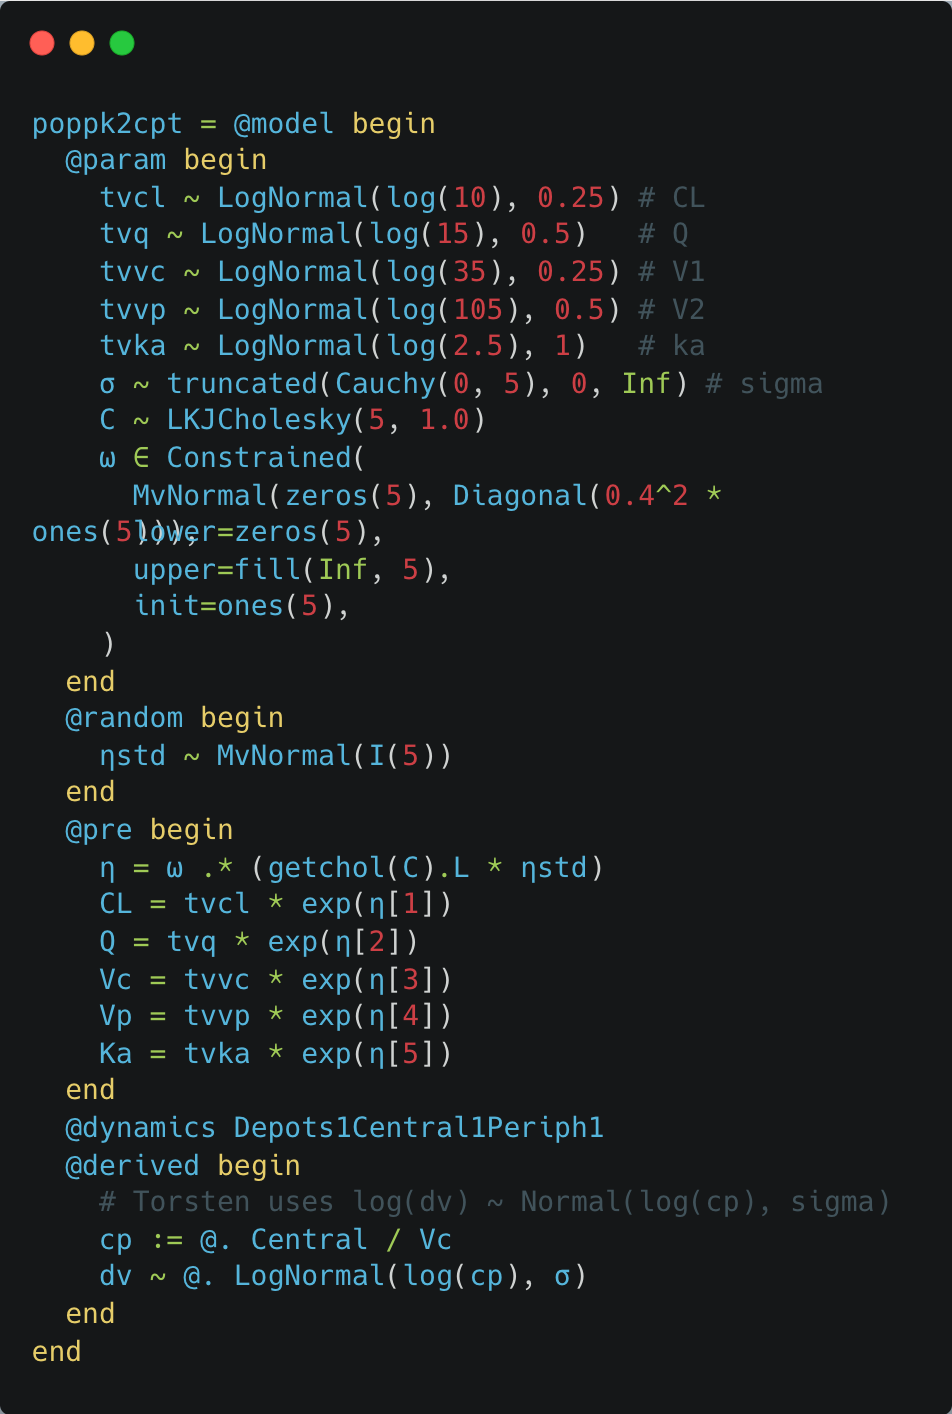
\includegraphics[width=0.3\columnwidth]{poppk2cpt.png}
\end{frame}
